\section{Allgemeines}
\begin{itemize}
    \item NO-SQL $\implies$ Not-Only-SQL
    \item Nicht relational, keine fixe Tabellenstruktur, erlauben horizontale Skalierung (= mehre Geräte statt stärkerer Hardware)
    \item Relationale Datenbanken kämpfen teils mit häufigen Änderungen an bestehenden Daten bzw. gigantischen Datenmengen
    \item Hauptattribute jeder Datenbank $\implies$ Konsistenz, Verfügbarkeit, Ausfalltoleranz $\implies$ CAP Theorem: Nicht alles kann zu 100\% erfüllt sein!
\end{itemize}
\begin{figure}[H]
    \centering
    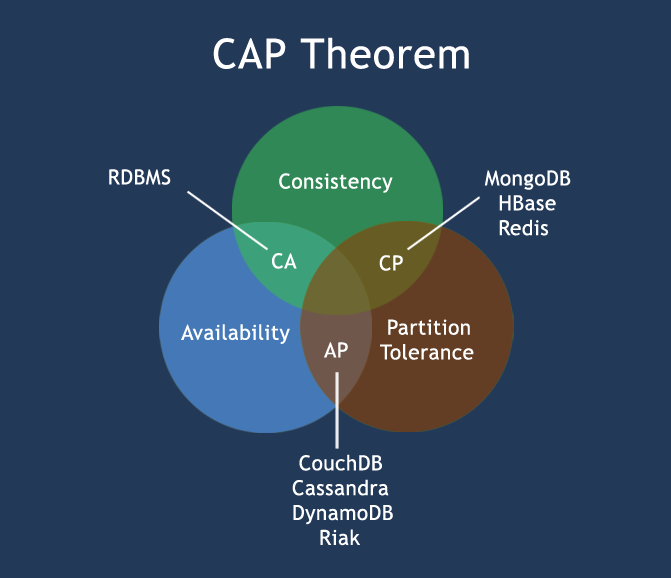
\includegraphics[scale=.4]{res/themenkorb_8/cap_theorem.png}
\end{figure}

\subsection{BASE}
\begin{itemize}
    \item NO-SQL Datenbanken arbeiten oft nach dem BASE-Prinzip
    \item Steht für Basically Available, Soft State, Eventual Consistency
    \item Gibt absolute Konsistenz der Daten auf, um dafür die Verfügbarkeit des Systems zu verbessern $\implies$ Kann zwischendurch in nicht konsistentem Zustand sein!
\end{itemize}

\subsection{Gliederung von NO-SQL Datenbanken}
\begin{itemize}
    \item Document-Store
    \begin{itemize}
        \item Kleinste Informationseinheit ist ein Document; wird mit einer eindeutigen ID identifiziert (meist automatisch generiert) $\implies$ z.B. MongoDB
    \end{itemize}
    \item Key-Value-Store
    \item Graph
    \begin{itemize}
        \item Daten werden in Knoten gespeichert, welche durch Kanten verbunden werden (können ebenfalls Informationen enthalten; z.B. Kosten der Verbindung)
        \item Speziell auf gewisse Queries ausgerichtet (Kürzester Pfad\dots)
    \end{itemize}
\end{itemize}